% section 1
% Kota Miura (miura@embl.de)

\section{Basics of Basics}

Handling of digital images in scientific research requires knowledge on
the characteristics of digital image. Signals we see in images are
quantitative information. We are taking pictures, but we are also
measuring signal by numbers. In this section, we learn the very basics
of the numerical nature of digital images. Inappropriate handling not
only lowers the quality of your analysis, but it could also be possible
that your processing is considered as the "manipulation
of data". For this latter point, please also refer to
\citet{Rossner2004}. There are some limits on image processing
to maintain the scientific validity. Standards on scientific image
processing could be found in "Digital Imaging:
Ethics" by \citet{cromey2007}. 

\subsection{Digital image is a matrix of numbers}
\label{subsec:imageEQmatrix}
Digital image we see on computer screen is made up of pixels. We can see
individual pixel by zooming up the image using magnifying tool\footnote{\
Zooming in / out of the image does not change the content of the image.}. Width
and height of the image are defined by the number of pixels in x and y
directions. Each pixel has brightness, or intensity (or more strictly,
amplitude) somewhere between black and white represented as a number. Within
image file saved in computer hard disk, intensity values of pixels are
written. The value is converted to the grayness of that pixel on monitor screen.
We usually do not see these values, or numbers, in the image displayed on
monitor, but we could access these numbers in the image file by converting 
the image file to a text file \footnote{It's also possible in a limited way by
putting mouse pointer over the image and checking the number indicated in
ImageJ menu bar.}.

\begin{indentexercise}{1}
\label{exer:1111}
\item Conversion of image to a text file
\item Make a new image by \ijmenu{[File > New > Image\ldots]}. In dialog window,
make a new image with the following parameters:

\begin{itemize}
\item name = test.txt
\item type = 8bit
\item Fill with Black
\item 10 pixel width
\item 15 pixel height
\item Slices = 1
\end{itemize}


%figure
\begin{figure}[htbp]
\begin{center}
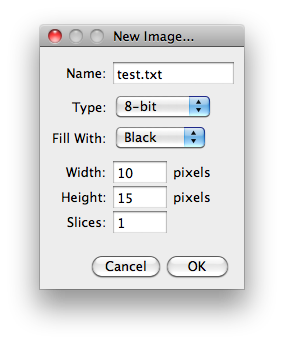
\includegraphics[width=5cm]{img/CMCIBasicCourse201102-img1.png}
\caption{ New Image Dialog}
\label{fig:img1}
\end{center}
\end{figure}
Clicking "OK", you will see a new window showing a black image (Fig.
\ref{fig:mostbasic}). At the top of the window you could see the file dimension ("10 x 15"), 
bit-depth and the file size (I explain these values later.
). Take the pen tool and draw some shape (what ever you want. 
If you do not see anything drawn, then you need to change the color of the pen to white by 
\ijmenu{[Edit > Option > Colors\ldots]} and set Foreground Color to white). 
Then do \ijmenu{[File > Save as > Text image]} and save the file. \\

You will find that the name of the file ends with ".txt". 
Open File Explorer (Win) or Finder (Mac) and double click the file. 
The file will be opened in text editor.

What you see now in the text editor is a "text image", a 2D
matrix of tab-delimited numbers. At the left most column in the example
(Fig. \ref{fig:mostbasic2}), there are only zeros. This corresponds to the left column
pixels in the image, where the color is black. In the middle in the
example image, there are several "255".
These are the white part of the image.
In the text image, edit one of the numbers (either 0 or 255) and change
to 100. Then save the file with a different name, such as
"temp.txt". Then in ImageJ open the file by \ijmenu{[File > Import > Text
Image\dots]}. You should see some difference in the image now. 
The image now has a dark gray dot, not black nor white.
\end{indentexercise}

%double figure
\begin{figure}[htbp]
\centering
\subfloat[]{\label{fig:img2}
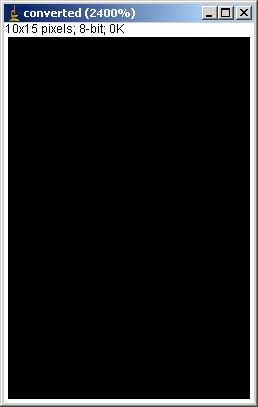
\includegraphics[width=3cm]{img/CMCIBasicCourse201102-img2.jpg}
}
\subfloat[]{\label{fig:img3}
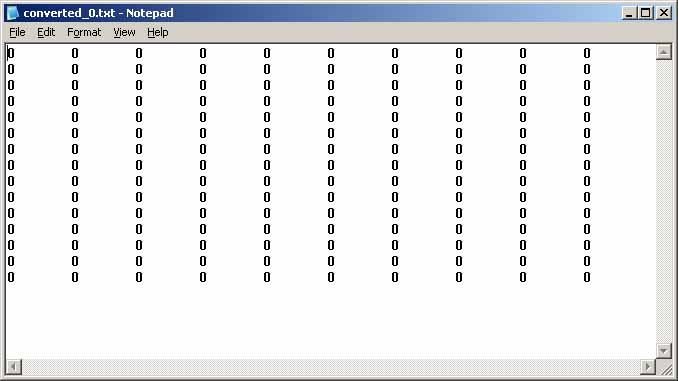
\includegraphics[width=9cm]{img/CMCIBasicCourse201102-img3.jpg}
}
\caption{ A digital image (b) is a matrix of numbers (b).}
\label{fig:mostbasic}
\end{figure} 

%double figure
\begin{figure}[htbp]
\centering
\subfloat[]{\label{fig:img4}
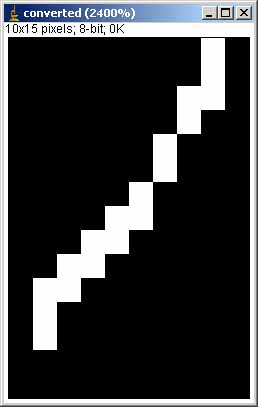
\includegraphics[width=3cm]{img/CMCIBasicCourse201102-img4.jpg}
}
\subfloat[]{\label{fig:img5}
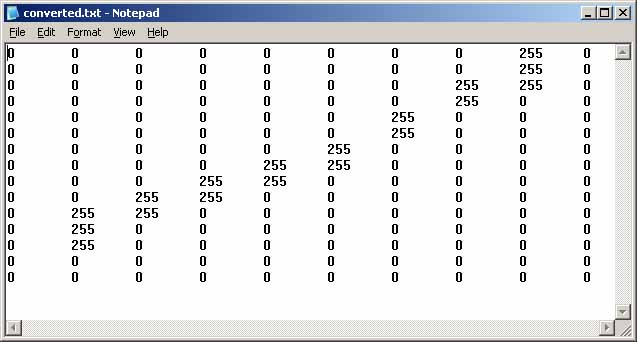
\includegraphics[width=9cm]{img/CMCIBasicCourse201102-img5.jpg}
}
\caption{ White line (a) corresponds to non-zero numbers (b).}
\label{fig:mostbasic2}
\end{figure} 


Note: In hard disk, pixel values are not written as a 2D matrix but as
a single array. Matrix is reproduced after loading according to the width
and height of the image. Pixel values of image stacks (3D or 4D), are
also in 1D array in hard disk. 3D or 4D matrix is reproduced according
to additional information such as slice and channel number. Such
information is written in the
"header" region of the file, which
precedes the "data" region of the
file where the 1D array of pixel array is contained. Header structure
is various depending on the file format, such as TIFF or BMP (we will
see more in "file formats and
header" section). 



\subsection{Image Bit-Depth}

Image file has a defined bit depth. You might have already
heard terms like "8-bit" or
"16-bit" and these are the bit depth. 8-bit
means that the gray-scale of the image has $2^{8} = 256$
steps: in other words, the grayness between black and white is divided
into 256 steps. 16-bit means $2^{16} = 65536$ steps. The
difference is that with 16-bit, one can assign gray-level much more
precise for each pixel; in other words "grayness
resolution" is higher. Microscope images are generated
mostly by CCD camera (or something similar, with matrix of
photo-sensor). CCD chip is a matrix of sensors. Each sensor receives
photons and converts the number received to the grayness number for a
pixel at the corresponding position within the image. Larger bit-depth
enables larger dynamic range with more precise conversion results.~ For
this reason, larger bit-depth is normally recommended for quantitative
imaging. Draw back is that it takes longer time for data transferring
as the bit-depth becomes larger. This may intern limits the time
resolution of image sequences. \\
~\\
Why do we use "$2^{n}$"? This
is because computer uses binary numbers. Minimum units are then 0 or 1.
8-bit means for example a number to be represented as 8-digits binary
number, something like "$00001010$" ( $= 10$ in
decimal). Then the minimum value is =
"$00000000$" ("0" in decimal) and the maximum is $11111111$
("255" in decimal). 8-bit image allows 256
scales for the grayness (using calculator application in your computer,
you could easily convert binary number into normal decimals and vice
versa). In case of 16-bit image, the scale is $2^{16}$ so
there are 65536 steps. 



We must keep in our mind that the nature is continuous. In conventional
mathematics you learn in school, decimal point enables you to represent
infinite steps between 0 and 1. But digitization of the nature loses
the infinite steps such that 0.44 will be rounded to 0 and 0.56 will be
1. Thus, the bit-depth limits the resolution of the analogue to digital
conversion (AD conversion). Higher bit depth generally allows higher
resolution.\\
\\
ImageJ has a high-bit-depth format called signed 32-bit floating point
image. In all above cases with 8-bit and 16-bit, the pixel value is
represented in integer but floating-point type enables decimal points
(real number) for the pixel value such as
"15.445". Though 32-bit floating point
image can be used for image calculation, many functions in ImageJ do
not~work properly so cares should be taken to use this image type. If
you want to know more about the 32-bit format, read the following box
(a bit complicated; you could just pass through)

\begin{quotation}
32 bit FLOATING POINT images utilizes efficient use of the 32 bits.
Instead of using 32 bits to describe 4,294,967,296 integer numbers, 23
bits are allocated to a fraction, 8 bits to an exponent, and 1 bit to a
sign, as follows:\\
~\\
$V = (-1)^{}S * 1.F * 2^{}(E-127)$,\\ 
whereby:\\
S = Sign, uses 1 bit and can have 2 possible values\\
F = Fraction, uses 23 bits and can have 8,388,608 possible
values\\
E = Exponent, uses 8 bits and can have 256 possible values\\
~\\
Practically speaking, this allows for an almost infinite number of tones
between level "0" and
"1", more than 8 million tones between
level "1" and
"2" and 128 tones between level
"65,534" and
"65,535", much more in line with our human
vision than a 32 bit integer image. Because of the infinitesimally
small numbers that can be stored, the 32 bit floating point format
allows to store a virtually unlimited dynamic range. In other words, 32
bit floating point images can store a virtually unlimited dynamic range
in a relatively compact way with more detail in the shadows than in the
highlights and take up only twice the size of 16 bits per channel
images, saving memory and processing power. A higher accuracy format
allows for smoother dynamic and tonal range compression.\\
\\
(Quote from \url{http://www.dpreview.com/learn/?/key=bits})
\end{quotation}




\subsection{Converting the bit-depth of image}

In many occasions, you might want to decrease the bit-depth of image
simply to reduce the file size (16-bit file becomes half the file size
when it is converted to 8-bit), or you might need to use certain
algorithm that is available only with 8-bit images (there are many such
cases), or so on. In any case, this will be a good experience for you
to see the limitation of bit-depth.

Here, we focus on the conversion of a 16-bit image to an 8-bit image to
study its effect and associated possible errors. 


\begin{indentexercise}{1}
Let's first open a 16-bit image from the sample. 
\ijmenu{[File > Open > m51.tif]}. Choose line selection tool and draw a vertical line 
(should be yellow by default: called line ROI). Then do \ijmenu{[Analyze > Plot Profile\ldots]}. 
A window pops up. See figures \ref{fig:img6} and \ref{fig:img7}.

\begin{figure}[htbp]
\begin{center}
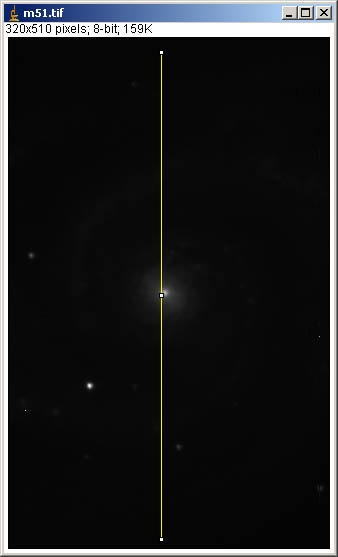
\includegraphics[width=5cm]{img/CMCIBasicCourse201102-img6.jpg}
\caption{Setting a vertical line Roi.}
\label{fig:img6}
\end{center}
\end{figure}

\begin{figure}[htbp]
\begin{center}
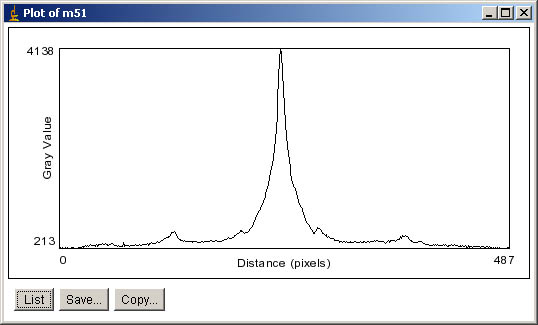
\includegraphics[width=5.694cm,height=3.44cm]{img/CMCIBasicCourse201102-img7.jpg}
\caption{profile of that ROI}
\label{fig:img7}
\end{center}
\end{figure}

Figure \ref{fig:img6} is the profile of the pixel values along the line ROI 
you just have marked on the image (Fig. \ref{fig:img7}). X-axis is the distance 
from the starting point (in pixel) and the y axis is the pixel value along the line ROI. 
The peak corresponds to the bright spot at the center of the image. 

Let's convert the image to 8-bit. First check the state
of "Conversion" option by
\ijmenu{[Edit > Option > Conversion]}. Be
sure that the checkbox "scale when
converting" is off. 

\begin{figure}[htbp]
\begin{center}
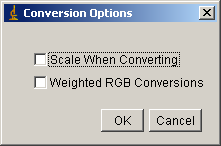
\includegraphics[width=5.847cm,height=3.863cm]{img/CMCIBasicCourse201102-img8.png}
\caption{Conversion Option. Scaling is turned off in this case. }
\label{fig:img8}
\end{center}
\end{figure}


Do \ijmenu{[Image > Type > 8-bit]}. The line
ROI is still there after the conversion. Do \ijmenu{[Analyze > Plot Profile\ldots] }again. 
You will find another graph pops up. Compare the previous profile (16-bit) and the new profile (8-bit).

Conversion causes changes in the y-value. Shapes of the profile look
mostly similar, so if you normalize two images, the curve may overlap.
This is because the image is scaled according to the following
formula.

\[
I_{8}(x,y) = \frac{I_{16}(x, y) - min(I_{16}(x,y))}{ max(I_{16}(x,y)) -  min(I_{16}(x,y))} *255
\]

where

$I_{16}(x, y)$: 16-bit image\\
$min(I_{16}(x,y))$: the minimum value of 16-bit image\\
$max(I_{16}(x,y))$: the maximum value of 16-bit image\\
$I_{8}(x, y)$: 8-bit image\\


Save the line ROI you created by \ijmenu{[Analyze Tools
ROI manager\ldots]}. A small dialog window pops up, so
click "Add" button in the right side.
Number appears in the left side, which indicates the name for the ROI
you made. ROI manager stores coordinates of the start / end points of
the line ROI.

Now, change the option \ijmenu{[Edit > Option >
Conversion]} that the checkbox "scale when
converting" is OFF. Open the 16-bit image again by
\ijmenu{[File > Open > m51.tif]}. Then
again, do \ijmenu{[Image > Type > 8-bit]}.
Apparent difference you see is that now the picture looks like a
overexpose image. Find the ROI manager window and click the ROI number
you stored in above. Same line ROI will appear in the new window. Then
do \ijmenu{[Analyze > Plot Profile\ldots]}. Third profile
shows very different shape compared to previous ones. This is because
the values above 255 is now considered as
"saturated", which means that what ever the
value is, numbers larger than 255 becomes 255.

%figure
\begin{figure}[H]
\begin{center}
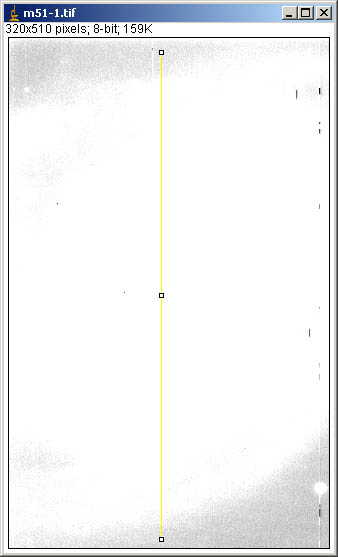
\includegraphics[width=5cm]{img/CMCIBasicCourse201102-img9.jpg}
\caption{ m51 image converted to 8-bit without scaling.}
\label{fig:img9}
\end{center}
\end{figure}

%double figure
\begin{figure}[H]
\centering
\subfloat[]{\label{fig:img10}
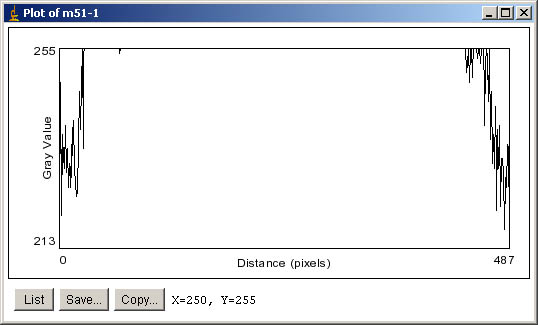
\includegraphics[width=5cm]{img/CMCIBasicCourse201102-img10.jpg}
}
\subfloat[]{\label{fig:img11}
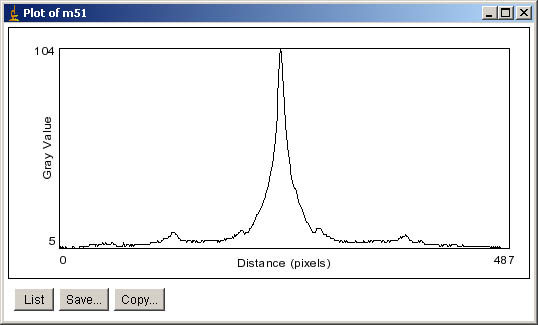
\includegraphics[width=5cm]{img/CMCIBasicCourse201102-img11.jpg}
}
\caption{ (a) Intensity profile of \ref{fig:img5}. If the conversion was done with scaling, then the profile would look like (b). }
\label{fig:8bitConverted}
\end{figure} 

\end{indentexercise}

When you do conversion, very different results could appear depending on
how you scale, like we have just seen. But in many cases, you do not
recognize such changes just by looking at the image: for this reason,
one should keep in mind that the conversion may
"saturate" or cause artifacts in the image
- screwing up scientific images to non-scientific ones. 


\subsection{Math functions}

Digital image is a matrix of numbers. We can calculate images like usual
math. If there is a flat image with pixel value of 10, and if you add 1
to the image, then all pixel values become 11. We think about a pixel
at $(5, 10)$, and we write down the calculation as follows:

\begin{equation}
f(5, 10) = 10
\end{equation}

\begin{equation}
g(5,10) = f (5, 10) +1 = 11
\end{equation}

We generalize this. x and y are the coordinates within the image.

\begin{equation}
g( x , y ) = f (x, y) + 1
\end{equation}

The original image is $f(x, y)$ and the result after the addition
is $g(x, y)$. 

Likewise images could also be subtracted, multiplied and divided by
number. 

\begin{indentexercise}{1}
Simple math on 8-bit image: Prepare a new
image following the initial part of the exercise \ref{exer:1111}. Now,
bring the mouse pointer over the image and check the
"value" that appears in the
status bar in the ImageJ window\footnote{\ In the exercise \ref{exer:1111}, 
we converted the image to a text file and check the pixel
values, but it is also possible to check the value pixel by pixel using
this method.}. All pixel values in the image should be
"value = 0".
"x=\ldots, y=\ldots " in the
status bar. 

Commands for mathematical operations in ImageJ are as follows. 

\ijmenu{[Process > Math > Add\ldots]}\\
\ijmenu{[Process > Math > Subtract\ldots]}\\ 
\ijmenu{[Process > Math > Multiply\ldots]} \\
\ijmenu{[Process > Math > Divide\ldots]}\\

%figure
\begin{figure}[htbp]
\begin{center}
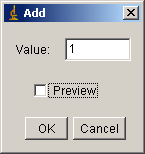
\includegraphics[width=3.8cm]{img/CMCIBasicCourse201102-img12.png}
\caption{ Add dialog.}
\label{fig:img12}
\end{center}
\end{figure}


Add 10 to the image: Do \ijmenu{[Process > Math > Add{\dots]}}. A dialog window pops up so you could
input 10. Press OK button. Now, place the mouse pointer over the image
to check that the pixel values actually became 10. Then select the pen
tool from the tool bar, and draw a diagonal line in the window. Check
again the pixel value. The line you just drew has pixel value 255. Then
add 10 again to the image by \ijmenu{[Process > Math > Add{\dots]}}. Check the pixels by placing the pointer.
The black part is now 20, but what happened to the white line? 

Since the image bit-depth is 8, the available number is only between 0
and 255. When you add 10 to a pixel with its value 255, the calculation
returns 255 because the number
"265" does not exist in 8-bit
world. The similar limitation applies for other calculations also. If
you multiply a pixel value 100 by 3, the answer in normal mathematics
is 300. But in 8-bit world, that pixel becomes 255. 

How about division? Close the currently working test image, and prepare
a new image as you did in \ref{subsec:imageEQmatrix}. Zoom up the image, and add 100
(\ijmenu{[Process > Math > Add{\dots]}}; you
should see the image turns to gray from black). Check pixel values by
placing the pointer above the image. Now, Divide the image by 3
(\ijmenu{[Process > Math > Divide{\dots]}}).
Check the result by placing the mouse over the image. The pixel value
is now 33. Since there is no decimal places in 8-bit, the division
returns the rounded value of (100 / 3 = 33). One could also divide
image by any real number, such as 3.1415. The answer will be in integer
in all cases in 8-bit and 16-bit. In case of floating point 32-bit
image, the calculation results are different. We study this in the next
exercise. 
\end{indentexercise}

\begin{indentexercise}{2}
Simple Math on 32-bit Image: prepare a new
32-bit image (in the \ijmenu{[New > Image..]} dialog,
select 32-bit from the "type"
drop-down menu). Then add 100 to the image. Check that the image pixel
values are all 100. Then divide the image by 3. Check the answer. This
time, answer has decimal places. 
\end{indentexercise}

Bit-depth limitation of digital image is very important for you to know,
in terms of quantitative measurements. Any measurement must be done
knowing the dynamic range of the detection system prior to the
measurement. \textit{If you are trying to measure the amount of
protein, and if some of the pixels are saturated, then your measurement
is invalid}. 

\subsection{Image Math }

In the precious section we calculated using single image. Likewise, we
can do calculation using two images. For example, if there are two
images with a same dimension, and 

\begin{equation}
f(5, 10) = 100
\end{equation}

\begin{equation}
g(5, 10) = 50
\end{equation}

\ldots meaning that the pixel value at the position $(5, 10)$ in the
first image \textit{f} is 100 and in the second image g is 50, we can
add these values and have a third image

\begin{equation}
h(5, 10) = f(5, 10) + g(5, 10) = 100 + 50 = 150
\end{equation}

General form is then as follows that applies to all pixels in the
image:

\begin{equation}
h(x, y) = f(x, y) + g(x, y)
\end{equation}

Note that this only works when the image width and height are
identical. Above is an example of addition. More numerical assignments
are available in ImageJ: \ 

\begin{center}
\tablehead{}
\begin{supertabular}{|m{4.748cm}|m{6.282cm}|}
\hline
\selectlanguage{english}\sffamily Add &
\selectlanguage{english}\sffamily img1 = img1+img2\\\hline
\selectlanguage{english}\sffamily Subtract &
\selectlanguage{english}\sffamily img1 = img1-img2\\\hline
\selectlanguage{english}\sffamily Multiply &
\selectlanguage{english}\sffamily img1 = img1*img2\\\hline
\selectlanguage{english}\sffamily Divide &
\selectlanguage{english}\sffamily img1 = img1/img2\\\hline
\selectlanguage{english}\sffamily AND &
\selectlanguage{english}\sffamily img1= img1 AND img2\\\hline
\selectlanguage{ngerman}\sffamily OR &
\selectlanguage{ngerman}\sffamily img1 = img1 OR img2\\\hline
\selectlanguage{ngerman}\sffamily XOR &
\selectlanguage{ngerman}\sffamily img1 = img1 XOR img2\\\hline
\selectlanguage{ngerman}\sffamily Min &
\selectlanguage{ngerman}\sffamily img1 = min(img1,img2)\\\hline
\selectlanguage{ngerman}\sffamily Max &
\selectlanguage{ngerman}\sffamily img1 = max(img1,img2)\\\hline
\selectlanguage{ngerman}\sffamily Average &
\selectlanguage{ngerman}\sffamily img1 = (img1+img2)/2\\\hline
\selectlanguage{ngerman}\sffamily Difference &
\selectlanguage{ngerman}\sffamily img1 =
{\textbar}img1-img2{\textbar}\\\hline
\selectlanguage{ngerman}\sffamily Copy &
\selectlanguage{ngerman}\sffamily img1 = img2\\\hline
\end{supertabular}
\end{center}


\begin{figure}[htbp]
\begin{center}
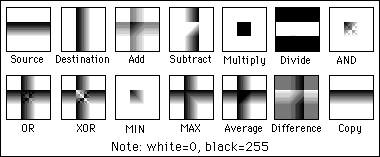
\includegraphics[width=10.945cm,height=4.323cm]{img/CMCIBasicCourse201102-img13.png}
\caption{Taken from ImageJ web site. \url{http://rsb.info.nih.gov/ij/docs/menus/process.html}}
\label{fig:img13}
\end{center}
\end{figure}

\begin{indentexercise}{1}
Image Math -- subtraction:\\
Open Images \textbf{cells\_ActinDNA.tif} and \textbf{cells\_Actin.tif}.
The first image is containing images from two channels. One is actin
labeled, and the other is DNA labeled. We isolate the DNA signal out of
the first image by image subtraction. Do \ijmenu{[Process > Image > Calculator\ldots]}. In the pop-up window, choose the appropriate combination to subtract \textbf{cells\_Actin.tif} from \textbf{cells\_ActinDNA.tif}. Don't forget to turn on the checkbox "Create New Window". 
\end{indentexercise}


\subsection{RGB image}

Color images are in RGB format (could also be so pseudo-color image, or
8-bit color, but this is just because of LUT. See section \ref{subsec:LUT}).
Another popular format is "CMKY" but this
format is optimized for printing purpose (you may have heard it already
when you want to print something in Photolab). RGB stands for three
primary colors. Red, Green and Blue. If all of them are bright at the
same intensity, then the color is white (or gray). If only red is
bright, then the color is red, and so on. A single RGB image thus has
three different channels. In other words, three layers of different
images are overlaid in a single RGB image. Each channel (layer) has a
bit depth of 8-bit. So a single RGB image is 24-bit image. For this,
the file size of color pics becomes three times larger than a grayscale
8-bit image. Don't save 16bit image in RGB format,
since you lose a lot of information, for automatic conversion from 16
to 8 bit takes place. 

\begin{indentexercise}{1}
Working with RGB image:
 
\item (a) Open the image \textbf{RGB\_cell.tif} by \ijmenu{[File > Open]}. Then split the color image to 3 different frames \ijmenu{[Image > Color > Split Channels]}. 

\item (b) Merge three frames by \ijmenu{[Image Color > Merge Channels\ldots]}. 

%figure
\begin{figure}[H]
\begin{center}
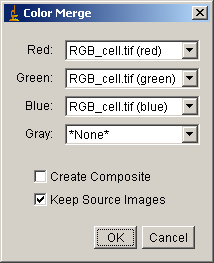
\includegraphics[width=5cm]{img/CMCIBasicCourse201102-img14.png}
\caption{ Color Merge Dialog}
\label{fig:img14}
\end{center}
\end{figure}

In the dialog window, choose an image name for each channel. Uncheck
"Create Composite" and check
"keep source images". Then try
swapping color assignments to see the effect. 

\item (c) Working on each channel separately: Close all windows and
open the "RGB\_cell.tif". Do
\ijmenu{[Image > Color > Channel Tools\ldots]}. Then click button "More" and select "Create Composite".
%figure
\begin{figure}[H]
\begin{center}
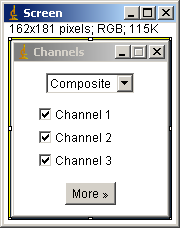
\includegraphics[width=4cm]{img/CMCIBasicCourse201102-img15.png}
\caption{ Channel Tool}
\label{fig:img15}
\end{center}
\end{figure}

Resulting image is a three-layer stack and each layer corresponds to one
of R, G or B. Each layer can be processed individually. 
%figure
\begin{figure}[H]
\begin{center}
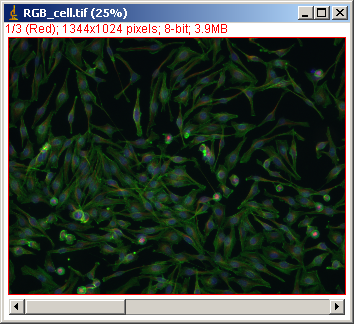
\includegraphics[width=9cm]{img/CMCIBasicCourse201102-img16.png}
\caption{ Composite image. Note slider at the bottom for switching between three channels.}
\label{fig:img16}
\end{center}
\end{figure}

Using Channel Tools again,
%figure
\begin{figure}[H]
\begin{center}
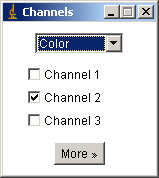
\includegraphics[width=4cm]{img/CMCIBasicCourse201102-img17.png}
\caption{ Channel Tool, now only selected for Channel 2.}
\label{fig:img17}
\end{center}
\end{figure}

Choose "color" from the pull-down tab, instead of "Composite". Select channel 2 (in this image, this will be Green channel). Select a part of the image using Rectangular ROI. 
%figure
\begin{figure}[H]
\begin{center}
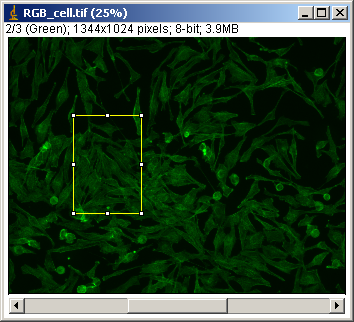
\includegraphics[width=9cm]{img/CMCIBasicCourse201102-img18.png}
\caption{ ROI selection, in channel 2. Note the position of slider.}
\label{fig:img18}
\end{center}
\end{figure}

Then do \ijmenu{[Edit > Clear]}. This will pop up a window. 
%figure
\begin{figure}[H]
\begin{center}
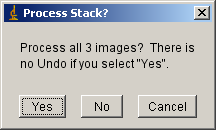
\includegraphics[width=4cm]{img/CMCIBasicCourse201102-img19.png}
\caption{ Asking you whether you want to process all channels.}
\label{fig:img19}
\end{center}
\end{figure}

Click No, because you want to process only one channel. 
%figure
\begin{figure}[H]
\begin{center}
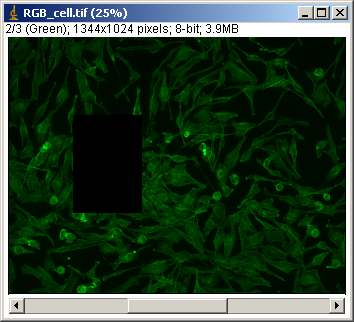
\includegraphics[width=9cm]{img/CMCIBasicCourse201102-img20.png}
\caption{ Channel 2 pixel values inside selected ROI becomes 0.}
\label{fig:img20}
\end{center}
\end{figure}
\begin{quote}
\textit{Troubleshooting}: If the ROI is not cleared (becomes bright), then you should change the background color setting. Do \ijmenu{[Edit > Option > Colors\dots]} and you will see a pop-up window like this. 
%figure
\begin{figure}[H]
\begin{center}
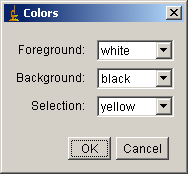
\includegraphics[width=4cm]{img/CMCIBasicCourse201102-img21.png}
\caption{ Color selection dialog.}
\label{fig:img21}
\end{center}
\end{figure}

Make sure that the background is "black". Do the ROI clearing again. 
\end{quote}
Select "Composite" in the pull-down tab of channel tool. 
%figure
\begin{figure}[H]
\begin{center}
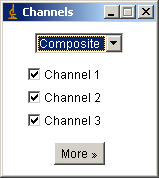
\includegraphics[width=4cm]{img/CMCIBasicCourse201102-img22.png}
\caption{ Choosing Composite, all channels visual.}
\label{fig:img22}
\end{center}
\end{figure}

Resulting image should look like below. 
%figure
\begin{figure}[H]
\begin{center}
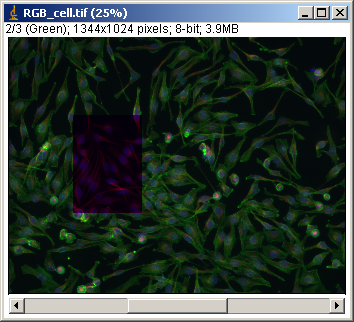
\includegraphics[width=9cm]{img/CMCIBasicCourse201102-img23.png}
\caption{ Only channel2 is devoid of image within the selected ROI.}
\label{fig:img23}
\end{center}
\end{figure}

In this case, green channel intensity in green channel ROI is now set to 0 ("clear"). You could do such
processing of single channel by simply selecting a channel by horizontal scroll bar and do the processing directly, such as drawing square ROI and deleting that part in that channel in "composite" view. 
\end{indentexercise}

\subsection{Look-Up Table }
\label{subsec:LUT}

We now look at how matrix of numbers is converted to actual image. Let"s think about a row of pixels with increasing pixel values from 0 to 255 (so there are 256 pixels in this row). Computer monitor will show a gradient of intensity that is linearly increasing its brightness from black to white. This is because the software is giving a command to the monitor, such that "this pixel $(x, y)$ is 158 so the corresponding voltage required for this position $(x, y)$ in the screen should be **mV". For this command to be composed, software needs a so called "look-up table" (LUT). 


This is just like a situation when you start checking a menu in a
restaurant with limited amount of money in your pocket. Say you want to
eat a pizza. You have only \texteuro 10 in your pocket. Looking at the
pizza menu, you will not try to find what you want from names of pizza
and what are the toppings, but instead you will check the prices listed
in the right side of the menu trying to figure out which pizza is less
then \texteuro 10. When you find \texteuro 7.5 in the list, then you slide your
sight to the left side of the menu, and find out that the pizza is
"Margherita". Similar to this,
software first checks the pixel value and then goes to the look-up
table (menu) to find out which brightness should be passed to the
monitor as a command ( = find a convincing price in the menu, then
sliding your sight to the left and find out which pizza to order).



\begin{indentexercise}{1}
For 8-bit images, there is a default LUT normally called "grayscale". To see the LUT, open the image \textbf{Cell\_Colony.jpg} and then do \ijmenu{[Image > Color > Show LUT]}. LUT window pops up showing the relationship between pixel value and pixel intensity. Try change the LUT by \ijmenu{[Image > Lookup Tables >Spectrum]}. Pixel value does not change by this operation, but the pixel intensity changes that the image appears differently now. Check the LUT again by do \ijmenu{[Image > Color > Show LUT]}. 
\end{indentexercise}

%double figure
\begin{figure}[H]
\centering
\subfloat[]{\label{fig:img24}
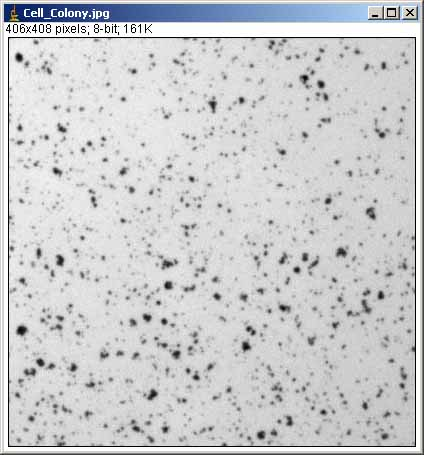
\includegraphics[width=6.371cm,height=6.853cm]{img/CMCIBasicCourse201102-img24.jpg}
}
\subfloat[]{\label{fig:img25}
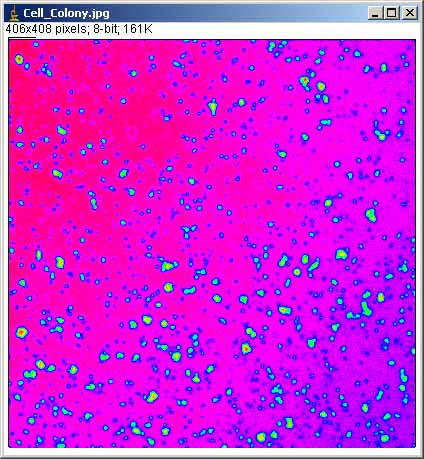
\includegraphics[width=6.431cm,height=6.962cm]{img/CMCIBasicCourse201102-img25.jpg}
}
\caption{ Grayscale LUT (a) converted to spectrum LUT (b).}
\label{fig:LUTconversionImages}
\end{figure} 

%double figure
\begin{figure}[H]
\centering
\subfloat[]{\label{fig:img26}
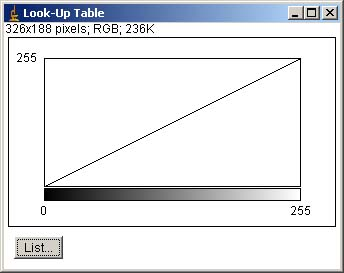
\includegraphics[width=6.055cm,height=4.805cm]{img/CMCIBasicCourse201102-img26.jpg}
}
\subfloat[]{\label{fig:img27}
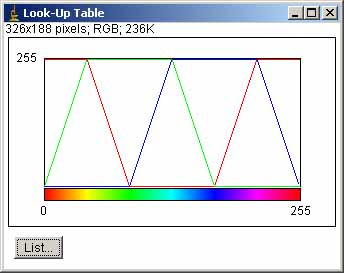
\includegraphics[width=6.103cm,height=4.833cm]{img/CMCIBasicCourse201102-img27.jpg}
}
\caption{ (a) Grayscale LUT and (b) spectrum LUT}
\label{fig:LUT[lots}
\end{figure} 

\subsection{Image File Formats: Header and Data, Stacks, Multi-dimensional images}

Image file contains two types of information. One is the image data, the matrix of numerical values. Another is called "header", which contains the information about the architecture of image. Since software must know information such as bit-depth, width and height, and the size of the header before opening the image, the information is written in the "header". The total file size of an image file is then 

$Total file size = header size + data size$

There are many different types of image formats, such as TIFF, BMP, PICT and so on. Each format has differently sized header, and also the location of the information. In biology, microscope companies create their own formats to include more parameters about the image, such as the type of microscope used, used objectives, binning, shutter speed, time intervals, user name and so on. 

Presence of company-specific formats complicates us because that image could only be openable from software provided by that company. For this reason, there are an excellent Plug-in which enable importing of specific format to ImageJ \footnote{\tab LOCI Bioformat Plugin:\\
\url{http://www.loci.wisc.edu/ome/formats.html}}

You do not have to know all the details about the architecture of various image formats (thanks to the bioformats plugin), but it is important for you to know that the difference resides mainly in the header. The data part is in most cases same, something like what we have seen already using text image (for more details on header, refer to the appendix \ref{app1} ). 

\textit{Multidimensional data}: When you take time-lapse images or z-stack, then there will be a series of images with same prefix and serial number like image0001.tif, image0002.tif, image0003.tif\dots\ and so on. These files could be imported by ImageJ and watch the sequence like a movie. Such an image series is called "stack" in ImageJ and can be saved as a single file. File extension is typically ".tif", which is same as the single frame file. In Metamorph, popular software used in biology, uses .stk as the file extension. These files can be loaded directly in ImageJ. We will study more on the actual use of the image stacks in section \ref{sec:timeseries}.

\textit{Compression}: Another important point that we must keep in our mind is that we should not compress data, if you want to get some numbers out of them. Popular compression formats are like JPEG and GIF. Compression of images deals with throwing away redundant part or mathematically interpolating some parts of the image. This causes artifacts in the image and it could even be "manipulation" of data. We must avoid using compression for the images we use for measurements. These compression formats are also called "lossy" formats, as the process of compression loses data. PNG is a compression format that does not alter the original pixel values.

\begin{indentexercise}{1}
Open the example image \textbf{wt1.tif}. Do
\ijmenu{[Image > Show Info\dots]}. Scale (pixels/inch)
is listed in the information window, which was read out from the header
of the image. Then do \ijmenu{[Image > Properties]},
also showing the scale. 
\end{indentexercise}

\subsection{Resizing images. (Shrinking and Enlarging) }

When we say "resizing" images, this
does not mean zooming in or out the image\footnote{\ Zooming is done by
the magnification tool (icon of magnification glass) and this simply
enlarges or shrinks the pixels, not modifying the original data. \par
}. Resizing changes the original data. If we have an image of size 10
pixels by 10 pixels and resize it to 200\%, the image becomes 20 x 20.
If we resize it by 50\%, then the image becomes 5 x 5. Resizing is a
simple task that could be done by \ijmenu{[Image > Adjust > Size\ldots]}. This is a simple operation but one must
take care about how pixels will be produced while enlarging and reduced
while shrinking. If the enlarging is simply two times larger, we could
imagine that each pixel will be copied three times to produce a block
of four pixels to complete the task. The pixel values of the newly
inserted pixels will then be identical to the source pixel. 

But what happens if we want to enlarge the image by 150 \%? To simplify
the situation, think about an image with 2 x 2 pixels. Then the
resulting image becomes 3 x 3. To understand the effect, do the
following exercise. 


\begin{indentexercise}{1}
Open the example image
4pixelimage\_sample.tif. The image is ultra small, so zoom it
up to the maximum (as much as you can, you must click on or
\textit{Ctrl - +}). You now see four pixels in the window.
Duplicate the image by \ijmenu{[Image > Duplicate]}.
Magnify again. "Select all" by
\ijmenu{[Edit > Selection > Select All]}.
Then \ijmenu{[Image > Adjust > Size\ldots]}.
In the dialog window, input the width 4 and height 4 (corresponds to
200\% enlargement). Turn on the check box "aspect
ratio" on and
"Interpolation" off. Then click
OK. Check the pixel values in original image, and the enlarged image.
\end{indentexercise}

\begin{indentexercise}{2}
Do the similar resizing, but this time enlarge
the image by 150\%. Check the pixel values.
%double figure
\begin{figure}[htbp]
\centering
\subfloat[]{\label{fig:img28}
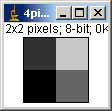
\includegraphics[width=3.951cm,height=3.916cm]{img/CMCIBasicCourse201102-img28.jpg}
}
\subfloat[]{\label{fig:img29}
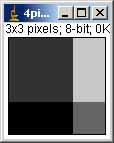
\includegraphics[width=4.022cm,height=5.045cm]{img/CMCIBasicCourse201102-img29.jpg}
}
\caption{ Artifacts produced by resizing. (a) Four pixel image and (b) nine pixel image after
resizing. }
\label{fig:resizing}
\end{figure} 

\end{indentexercise}

The resizing in the exercise was without interpolation -- the check box
was OFF. Interpolation is similar to the one dimensional interpolation
we do with graphs. In case of images, the gradient is also two
dimensional so the situation is a bit more complex. There are various
methods for interpolating image. The interpolation method used in
ImageJ is the \textit{bilinear interpolation}. Briefly, the bilinear
interpolation algorithm samples pixel values in the surrounding of the
insertion point, and calculates the pixel value for that
position\footnote{\ For more details on bilinear interpolation, refer
to\\
http://www.cambridgeincolour.com/tutorials/image-interpolation.htm.}.
One must keep in mind that the result of enlarging or shrinking of
image depends on the interpolation method -- and scientific results
could be altered depending on the method you use.

\clearpage
\subsection{ASSIGNMENTS }%%%%%%%%%%%%%%%%%%%%%%%

\textbf{\sffamily
Assignment 1-1-1: Digital image = matrix of numbers}

Edit a text image using text editor. Be sure to insert space between
numbers as separator. Save the text file and open it as an image in
ImageJ by importing text image function. \ \ 

\textbf{\sffamily
Assignments 1-1-2: bit depth}
\begin{enumerate}
\item How many gray scale steps does a 12-bit image have?\\
\item Describe in text how a 1-bit image looks like.
\end{enumerate}

\textbf{\sffamily
Assignment 1-1-3: bit depth conversion}

Use m51.tif (16-bit!) sample image to draw a plot profile, as we did in
the course. In the profile plot window, a
"list" button is at the left-bottom corner.
Click the button. You will then see a new window containing a column on
numbers. These numbers can be copy \& pasted to spread sheet software
such as Openoffice Calc or MS Excel. Overlay three curves in a graph,
and discuss the difference in two different ways of bit-conversions. 

\textbf{\sffamily
Assignments 1-1-4: Simple math with Image}
\begin{enumerate}
\item Try subtracting certain values from the image you created in
the Assignment 1-1-1 and check that the values cannot be less than 0. 
\item Prepare an 8-bit image with pixel value 200. Divide the
image by 3, and check the answer. 

\item Prepare a 16-bit image. In the \ijmenu{[File > New > 
Image\ldots]} dialog, select 16-bit from the
"type" drop-down menu. Try adding
certain value to check the maximum pixel value. 

\item Discuss why measurement of fluorescence intensity using
digital image is invalid when some pixels are saturated. 
\end{enumerate}

\textbf{\sffamily
Assignments 1-1-5: LUT}

Open "Cell\_Colony.tif". Use LUT edit function and design your own LUT to highlight the black dots in
Green and the background in Black. "LUT editor" can be activated by \ijmenu{[Images > Color > Edit LUT\ldots]}. Instruction for the LUT editor is at\\
\url{http://rsb.info.nih.gov/ij/plugins/lut-editor.html} \\
You might be able to manage using it without reading the web instruction; just try!). LUT (.lut file) could also be edited using Excel. 

\textbf{\sffamily
Assignments 1-1-6: File size and image bit depth, image size}

If there is an image with width = 100 pixels and height = 200 pixels,
what would be the expected size of the image file in bytes? 1 byte =
8-bit.

Create a new image with the dimension as above, and save the image in
"bitmap (.bmp)" format and check the file
size. Is it same as you expected, or different? Save the same image in
text file format and check the file size again.

\textbf{\sffamily
Assignment 1-1-7 Resizing}

\begin{enumerate}
\item Enlarge the sample image 4pixelimage\_sample.tif by
150\% while the "Interpolation"
check box in the size adjustment window is ON. Study the pixel values
before and after the enlargement. What happened? Describe the result.

\item Change "canvas size" by \ijmenu{[Image > Adjust > Canvas Size]} for any image. What"s the
difference to "Resize"?
\end{enumerate}


